\documentclass{article}

\usepackage[letterpaper, margin=1.3cm]{geometry}
\usepackage[utf8]{inputenc}
\usepackage{siunitx}
\usepackage{mathtools}
\usepackage{multicol}
\usepackage[RPvoltages, american, betterproportions, siunitx]{circuitikz}
\usepackage{gensymb}

\title{ECE 203 Problem Set 7}
\author{Michael Kwok}
\date{March 2020}
\begin{document}

\maketitle
\begin{multicols}{2}
\section*{1}
\subsection*{a}

\begin{align*}
10 \cdot \frac{10}{25} &= \SI{4}{\volt}\\
V_b &= \SI{4}{\volt}\\
V_a &= V_b = V_c = \SI{4}{\volt}\\
\frac{\SI{4}{\volt}}{\SI{2000}{\ampere}} &\cdot \SI{1000}{\ohm} = \SI{2}{\volt}
\end{align*}

\subsection*{b}

\begin{align*}
\left(\frac{1}{10} + \frac{1}{2}\right)^{-1} &= \frac{5}{3}\\
\frac{10\cdot\frac{5}{3}}{15+\frac{5}{3}} &= \SI{1}{\volt}\\
V_x = \frac{1}{2} &= \boxed{\SI{0.5}{\volt}}
\end{align*}

\subsection*{c}
\begin{align*}
    V_b &= \SI{4}{\mega\ohm} \cdot \SI{1}{\micro\volt}\\
    &= \SI{4}{\volt}
\end{align*}
\subsection*{d}
Part A:
\begin{align*}
    V_x &= \SI{2}{\volt}\\
    I_{out} &= \frac{V_x}{\SI{1000}{\ohm}}\\
    &= \SI{2}{\milli\ampere}
\end{align*}
Part C:
$$
I_{out} = \frac{21.1}{75000} + 0.001 = \SI{1.28}{\milli\ampere}
$$
\section*{2}
\subsection*{a}
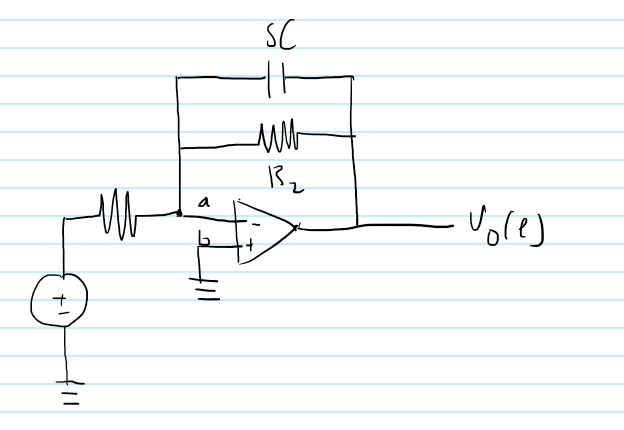
\includegraphics[scale=0.5]{PS7cct.png}
\begin{align*}
V_a &= V_b = 0\\
Z_{oa} &= \left( sC + \frac{1}{R_2}\right)^{-1}\\
&= \left( \frac{sCR_2 + 1}{R_2}\right)^{-1}\\
&= \frac{R_2}{sCR_2+1}\\
-V_o &+ I_o Z_{oa} + R_1 I_o + V_s = 0\\
V_o &= I_o Z_{oa}\\
\end{align*}
\begin{align*}
    R_1 I_o + V_s &= 0\\
    V_s &= -R_1 I_o\\
    V_s &= -R_1 \frac{V_o}{Z_{oa}}\\
    H(s) &= -\frac{Z_{oa}}{R_1}\\
    &= -\frac{R_2}{R_1}\left(\frac{1}{sCR_2 + 1}\right)
\end{align*}
\subsection*{b}
\begin{align*}
V_m &= 1\\
s &= 0
\end{align*}
\begin{align*}
    \tilde{V}_{of} &= H(s) \tilde{V}(s) = -\frac{100000}{10000}\\
    &= -\SI{10}{\volt}\\
    V_{of}(t) &= -\SI{10}{\volt}\\
\end{align*}
\subsection*{c}
$$
    -\frac{100\times 10^3}{10s+10000}
$$
No zero, pole at $s = -\frac{1000}{10} = -1000$
$$
V_{on} = A e^{-1000t}
$$
\subsection*{d}
$$
V_o (t) = A e^{-1000t} - 10
$$
\section*{3}
\subsection*{a}
\begin{align*}
    \tilde{V}_b &= \frac{R \tilde{V}_s}{R+\frac{1}{j\omega C}}\\
    \tilde{V}_a &= \tilde{V}_s + \frac{R_1\tilde{V}_o - \tilde{V}_s}{2R_1}\\
    &= \tilde{V}_s + \frac{\tilde{V}_o - \tilde{V}_s}{2}\\
    \frac{R \tilde{V}_s}{R+\frac{1}{j\omega C}} &= \tilde{V}_s + \frac{\tilde{V}_o - \tilde{V}_s}{2}\\
    2R\tilde{V}_s = 2 \tilde{V}_s \left( R + \frac{1}{sC} \right) &+ \left(\tilde{V}_o - \tilde{V}_s\right)\left(R+\frac{1}{sC}\right)\\
    \tilde{H}(s) &= \frac{R-\frac{1}{sC}}{R+\frac{1}{sC}}\\
    &= \frac{sCR-1}{sCR+1}\\
    &= \frac{j\omega CR-1}{j\omega CR+1}
\end{align*}
\subsection*{b}
\begin{align*}
    \tilde{H}(j\omega) &= \frac{j\omega\cdot 0.01\times 10^{-6}\cdot 20\times10^3 -1}{j\omega\cdot 0.01\times 10^{-6}\cdot 20\times10^3+1}\\
    &= \frac{j-1}{j+1} = \frac{(j-1)^2}{-1-1} = \frac{-2j}{-2}
\end{align*}
\begin{align*}
    |\tilde{H}(j\omega)| &= 1\\
    \angle \tilde{H}(j\omega) &= +90\degree
\end{align*}
\end{multicols}
\end{document}
